\documentclass[aspectratio=169,11pt]{beamer}

% --- pdflatex-compatible, self-contained (no fontspec/metropolis) ---
\usepackage[T1]{fontenc}
\usepackage{lmodern}
\usepackage{booktabs}
\usepackage{tikz}
\usetikzlibrary{arrows.meta,positioning,shapes.geometric}
\usepackage{xcolor}
\usepackage{graphicx}
\graphicspath{{../results/figures/}{../results/figures/candidates/}{../results/figures/validation/}{../results/figures/reorg/}{../results/figures/pipeline/}{figures/}}

% --- clean modern theme built on defaults ---
\usetheme{default}
\usefonttheme{professionalfonts}
\setbeamertemplate{navigation symbols}{}
\setbeamertemplate{itemize items}[circle]

\definecolor{ink}{HTML}{15304A}      % deep blue
\definecolor{teal}{HTML}{0E7C86}     % accent
\definecolor{amber}{HTML}{E08A1E}    % highlight
\definecolor{good}{HTML}{2E7D32}     % green
\definecolor{bad}{HTML}{C0392B}      % red
\definecolor{soft}{HTML}{F2F5F7}

\setbeamercolor{frametitle}{fg=white,bg=ink}
\setbeamercolor{title}{fg=ink}
\setbeamercolor{structure}{fg=teal}
\setbeamercolor{block title}{fg=white,bg=teal}
\setbeamercolor{block body}{bg=soft}
\setbeamerfont{frametitle}{series=\bfseries}
\setbeamertemplate{frametitle}{%
  \nointerlineskip
  \begin{beamercolorbox}[wd=\paperwidth,ht=3.2ex,dp=1.2ex,leftskip=0.35cm,rightskip=0.35cm]{frametitle}%
    \bfseries\insertframetitle%
  \end{beamercolorbox}%
}
\setbeamertemplate{footline}{\hfill\scriptsize\textcolor{ink!60}{\insertframenumber}\hspace{2ex}\vspace{1ex}}

\newcommand{\good}[1]{\textcolor{good}{\textbf{#1}}}
\newcommand{\bad}[1]{\textcolor{bad}{\textbf{#1}}}
\newcommand{\hi}[1]{\textcolor{amber}{\textbf{#1}}}

\title{\textbf{Computational Screening of Redox-Active Monomers}}
\subtitle{A physics-based, multi-objective candidate-selection pipeline}
\author{RTFB Materials Research}
\date{\today}

\begin{document}

% ---------------------------------------------------------------
\begin{frame}[plain]
  \titlepage
  \begin{center}\small\textcolor{ink!70}{Redox potential $\cdot$ Stability $\cdot$ Kinetics $\cdot$ Capacity}\end{center}
\end{frame}

% ---------------------------------------------------------------
\begin{frame}{The goal: pick good redox molecules for flow batteries}
  \begin{columns}[T]
    \begin{column}{0.56\textwidth}
      \textbf{System.} A \hi{Merrifield-resin polymer} carrying pendant redox groups.
      The redox chemistry is \emph{local}, so we model the \hi{monomer as a proxy}:
      establish we can capture the local chemistry, then add backbone effects.
      \vspace{1.5ex}

      \textbf{Selection is multi-objective.} Voltage and stability are necessary but not
      sufficient:
      \[
        \text{Energy density} \propto n \cdot V_\text{cell} \cdot \text{solubility}
      \]
      \vspace{-1ex}
      \begin{itemize}
        \item \textbf{redox potential} $\rightarrow$ cell voltage / window
        \item \textbf{stability} $\rightarrow$ cycle life
        \item \textbf{kinetics} ($\lambda$), \textbf{capacity} ($n$), cost, crossover
      \end{itemize}
    \end{column}
    \begin{column}{0.42\textwidth}
      \begin{block}{Guiding principle}
        Energy \emph{differences} with error cancellation compute \good{reliably};
        \emph{absolute} charged-species solvation does \bad{not}.
        \\[1ex]
        Build objectives on the cancellation-friendly quantities; treat the rest as
        labelled proxies or filters.
      \end{block}
    \end{column}
  \end{columns}
\end{frame}

% ---------------------------------------------------------------
\begin{frame}{The pipeline (per redox state)}
  \begin{center}
  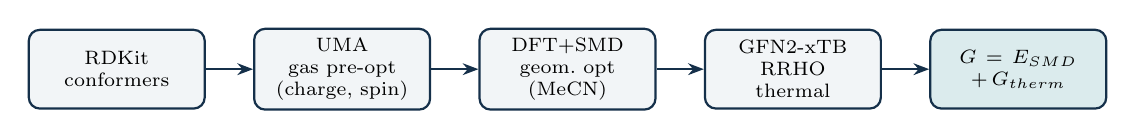
\begin{tikzpicture}[
      node distance=6mm,
      box/.style={rectangle,rounded corners,draw=ink,fill=soft,thick,
                  minimum height=10mm,text width=20mm,align=center,font=\scriptsize},
      arr/.style={-{Stealth[length=2mm]},thick,ink}]
    \node[box] (a) {RDKit\\conformers};
    \node[box,right=of a] (b) {UMA\\gas pre-opt\\(charge, spin)};
    \node[box,right=of b] (c) {DFT+SMD\\geom.\ opt\\(MeCN)};
    \node[box,right=of c] (d) {GFN2-xTB\\RRHO\\thermal};
    \node[box,right=of d,fill=teal!15] (e) {$G = E_\text{SMD}$\\$+\,G_\text{therm}$};
    \draw[arr] (a)--(b); \draw[arr] (b)--(c); \draw[arr] (c)--(d); \draw[arr] (d)--(e);
  \end{tikzpicture}
  \end{center}
  \vspace{1ex}
  \begin{columns}[T]
    \begin{column}{0.5\textwidth}
      \footnotesize
      \textbf{Level of theory}
      \begin{itemize}\footnotesize
        \item opt: r$^2$SCAN/def2-SVP(D) + SMD
        \item energy: $\omega$B97M-V/def2-TZVP
        \item referenced to level-matched Fc/Fc$^+$
      \end{itemize}
    \end{column}
    \begin{column}{0.5\textwidth}
      \footnotesize
      \textbf{Two hard-won fixes}
      \begin{itemize}\footnotesize
        \item gpu4pyscf open-shell Hessian is \bad{broken}
              $\rightarrow$ thermal from \hi{GFN2-xTB} RRHO
        \item cross-points gas-only (\texttt{do\_smd=False}), $\sim$2$\times$ cheaper
      \end{itemize}
    \end{column}
  \end{columns}
\end{frame}

% ---------------------------------------------------------------
\begin{frame}{How each axis is computed}
  \footnotesize
  \begin{table}
  \renewcommand{\arraystretch}{1.15}
  \begin{tabular}{@{}p{2.5cm}p{5.4cm}p{3.5cm}@{}}
    \toprule
    \textbf{axis} & \textbf{method} & \textbf{validation / trust} \\
    \midrule
    redox potential & DFT+SMD $\Delta G$; $\omega$B97M-V/def2-TZVP\,//\,r$^2$SCAN/def2-SVP(D);
                      level-matched Fc ref & OROP exp: MAE 0.58 V, $\rho$ 0.95 \\
    thermal $G_\text{therm}$ & GFN2-xTB RRHO (298 K) & open-shell safe \\
    stability (disprop.) & $\Delta G_\text{disp}=F(E_\text{hi}-E_\text{lo})$ from state $G$'s
                      & exp spacings: MAE 0.17 eV, $\rho$ 1.0 \\
    stability (dimer.) & pimer cluster DFT+SMD $\Delta G$ & \bad{flagged} (+2 desolvation) \\
    reorg.\ energy $\lambda$ & $\lambda_i$ 4-point (Nelsen), gas $+\ \lambda_o$ (Marcus/Born, Eq.\,13) & D3TaLES $\lambda_i$: \good{$R^2{=}1.0$} ($n{=}2636$) \\
    reversibility & bond-graph change + solvated EA & catches dissoc.\ (CCl$_4$) \\
    capacity & $n\!\cdot\!F/\text{MW}$ (accessible $n$) & \good{exact} \\
    solubility & $\Delta G_\text{solv}=E_\text{SMD}-E_\text{gas}$ (neutral) & proxy (relative) \\
    synth.\ access. & RDKit SA\_Score & heuristic proxy \\
    \bottomrule
  \end{tabular}
  \end{table}
  \vspace{0.5ex}
  \centering\footnotesize
  \textcolor{ink!70}{Geometries optimized in SMD(MeCN); conformers via RDKit + UMA pre-opt.}
\end{frame}

% ---------------------------------------------------------------
\begin{frame}{Redox potential: benchmarked vs.\ experiment (OROP)}
  \begin{columns}[T]
    \begin{column}{0.5\textwidth}
      \textbf{Blind test on OROP MeCN potentials} ($n=36$):
      \begin{table}\footnotesize
      \begin{tabular}{lcc}
        \toprule
         & ours & OROP impl.-DFT \\
        \midrule
        MAE (V)        & 0.58 & 0.43 \\
        signed bias    & $+0.46$ & --- \\
        Spearman (all) & \good{0.95} & --- \\
        \bottomrule
      \end{tabular}
      \end{table}
      \vspace{1ex}
      Absolute accuracy sits at the \hi{$\sim$0.5--0.9 V physics floor} of implicit-solvent
      DFT --- the same for everyone. \good{Ranking}, not absolute potential, is the usable
      output.
    \end{column}
    \begin{column}{0.5\textwidth}
      \textbf{Ranking must be judged \emph{within} charge class}
      \begin{table}\footnotesize
      \begin{tabular}{lccc}
        \toprule
        class & $n$ & MAE & Spearman \\
        \midrule
        cations ($+1$)  & 21 & 0.44 & \good{0.885} \\
        anions ($0$)    & 13 & 0.77 & \bad{0.489} \\
        anions (filtered) & 8 & 0.53 & \good{0.952} \\
        \bottomrule
      \end{tabular}
      \end{table}
      \vspace{1ex}
      \footnotesize Global 0.95 is inflated (charge classes separate). Cations rank well;
      anions needed a fix $\rightarrow$ next slide.
    \end{column}
  \end{columns}
\end{frame}

% ---------------------------------------------------------------
\begin{frame}{The anion ``failure'' was category errors, not bad physics}
  \begin{columns}[T]
    \begin{column}{0.54\textwidth}
      The anion ranking collapse (Spearman 0.49) traced to a few molecules with
      \bad{no reversible reduction}:
      \begin{table}\footnotesize
      \begin{tabular}{llc}
        \toprule
        molecule & exp & RMSD$_\text{neu$\to$an}$ \\
        \midrule
        CCl$_4$    & $-2.57$ & \bad{3.4 \AA} \\
        CH$_2$Br$_2$ & $-3.12$ & 1.3 \AA \\
        (unbound anions) & --- & EA$_\text{gas}<0$ \\
        \bottomrule
      \end{tabular}
      \end{table}
      Dissociative electron attachment (CCl$_4$+e$^-\!\to$CCl$_3^{\bullet}$+Cl$^-$) ---
      scored against irreversible \emph{peak} potentials.
    \end{column}
    \begin{column}{0.46\textwidth}
      \begin{block}{Reversibility screen}
        Bound anion (solvated EA $>0$) \emph{and} intact (\hi{bond-graph unchanged}, not
        raw RMSD --- which is confounded by tether flexibility).
      \end{block}
      \vspace{-0.5ex}
      \begin{itemize}\footnotesize
        \item filtering $\rightarrow$ anion Spearman \bad{0.49}$\rightarrow$\good{0.95}
        \item a \emph{required} screening criterion + a \emph{stability} signal
        \item all 20 candidate couples: \good{reversible}
      \end{itemize}
    \end{column}
  \end{columns}
\end{frame}

% ---------------------------------------------------------------
\begin{frame}{Stability = decomposition free energies}
  \begin{columns}[T]
    \begin{column}{0.54\textwidth}
      \textbf{Disproportionation} $2R \!\rightarrow\! R^{+}\!+R^{-}$ \\ (atom- \&
      electron-conserving $\rightarrow$ \good{cancellation $\rightarrow$ reliable}):
      \begin{table}\footnotesize
      \begin{tabular}{lr}
        \toprule
        intermediate & $\Delta G_\text{disp}$ (kJ/mol) \\
        \midrule
        TEMPO$^{\bullet}$          & \good{$+221$} \\
        AQ semiquinone             & $+86$ \\
        viologen MV$^{+\bullet}$   & $+52$ \\
        \bottomrule
      \end{tabular}
      \end{table}
      \footnotesize TEMPO --- the textbook persistent radical (our validation anchor) ---
      ranks most stable, as it must. Exact from existing energies; no new calculation.
    \end{column}
    \begin{column}{0.46\textwidth}
      \textbf{Dimerization} $2\,\text{MV}^{+\bullet}\!\rightarrow[\text{MV}_2]^{2+}$
      (the real viologen failure mode):
      \begin{block}{$\Delta G_\text{dim} = +0.49$ eV \ (flagged)}
        Config sampling: minimum well-defined ($\sigma_\text{config}\!\approx$ 2 meV).
        \\ The uncertainty is the \bad{$+2$ pimer desolvation} --- the continuum's weak spot.
      \end{block}
      \vspace{-0.5ex}
      \footnotesize $\Rightarrow$ use dimerization as a \hi{relative} ranking; lean on
      disproportionation as the trustworthy axis.
    \end{column}
  \end{columns}
\end{frame}

% ---------------------------------------------------------------
\begin{frame}{Kinetics: reorganization energy $\lambda=\lambda_i+\lambda_o$}
  \begin{columns}[T]
    \begin{column}{0.42\textwidth}
      \footnotesize
      \textbf{Inner-sphere} $\lambda_i$ --- solute geometry relaxation, \textbf{4-point (Nelsen)}:
      \[\lambda_i=[E_O(q_R)\!-\!E_O(q_O)]+[E_R(q_O)\!-\!E_R(q_R)]\]
      gas single points; \emph{identical} to D3TaLES. \good{Validated}.
      \vspace{1.2ex}

      \textbf{Outer-sphere} $\lambda_o$ --- solvent reorganization (Marcus/Born, \hi{Sharma Eq.\,13}):
      \[\lambda_o=\frac{z^2e^2}{8\pi\varepsilon_0 r_\text{hyd}}\!\left(\frac{1}{\varepsilon_\text{op}}-\frac{1}{\varepsilon_r}\right)\]
      MeCN ($\varepsilon_r{=}37.5,\ \varepsilon_\text{op}{=}1.81$); SASA $r_\text{hyd}$ proxy $\Rightarrow$
      \hi{semi-quantitative} ($\sim$2$\times$).
      \vspace{1.2ex}

      $\lambda_\text{total}=\lambda_i+\lambda_o$: trust $\lambda_i$; read $\lambda_o$ as \emph{relative}.
    \end{column}
    \begin{column}{0.58\textwidth}
      \begin{center}
      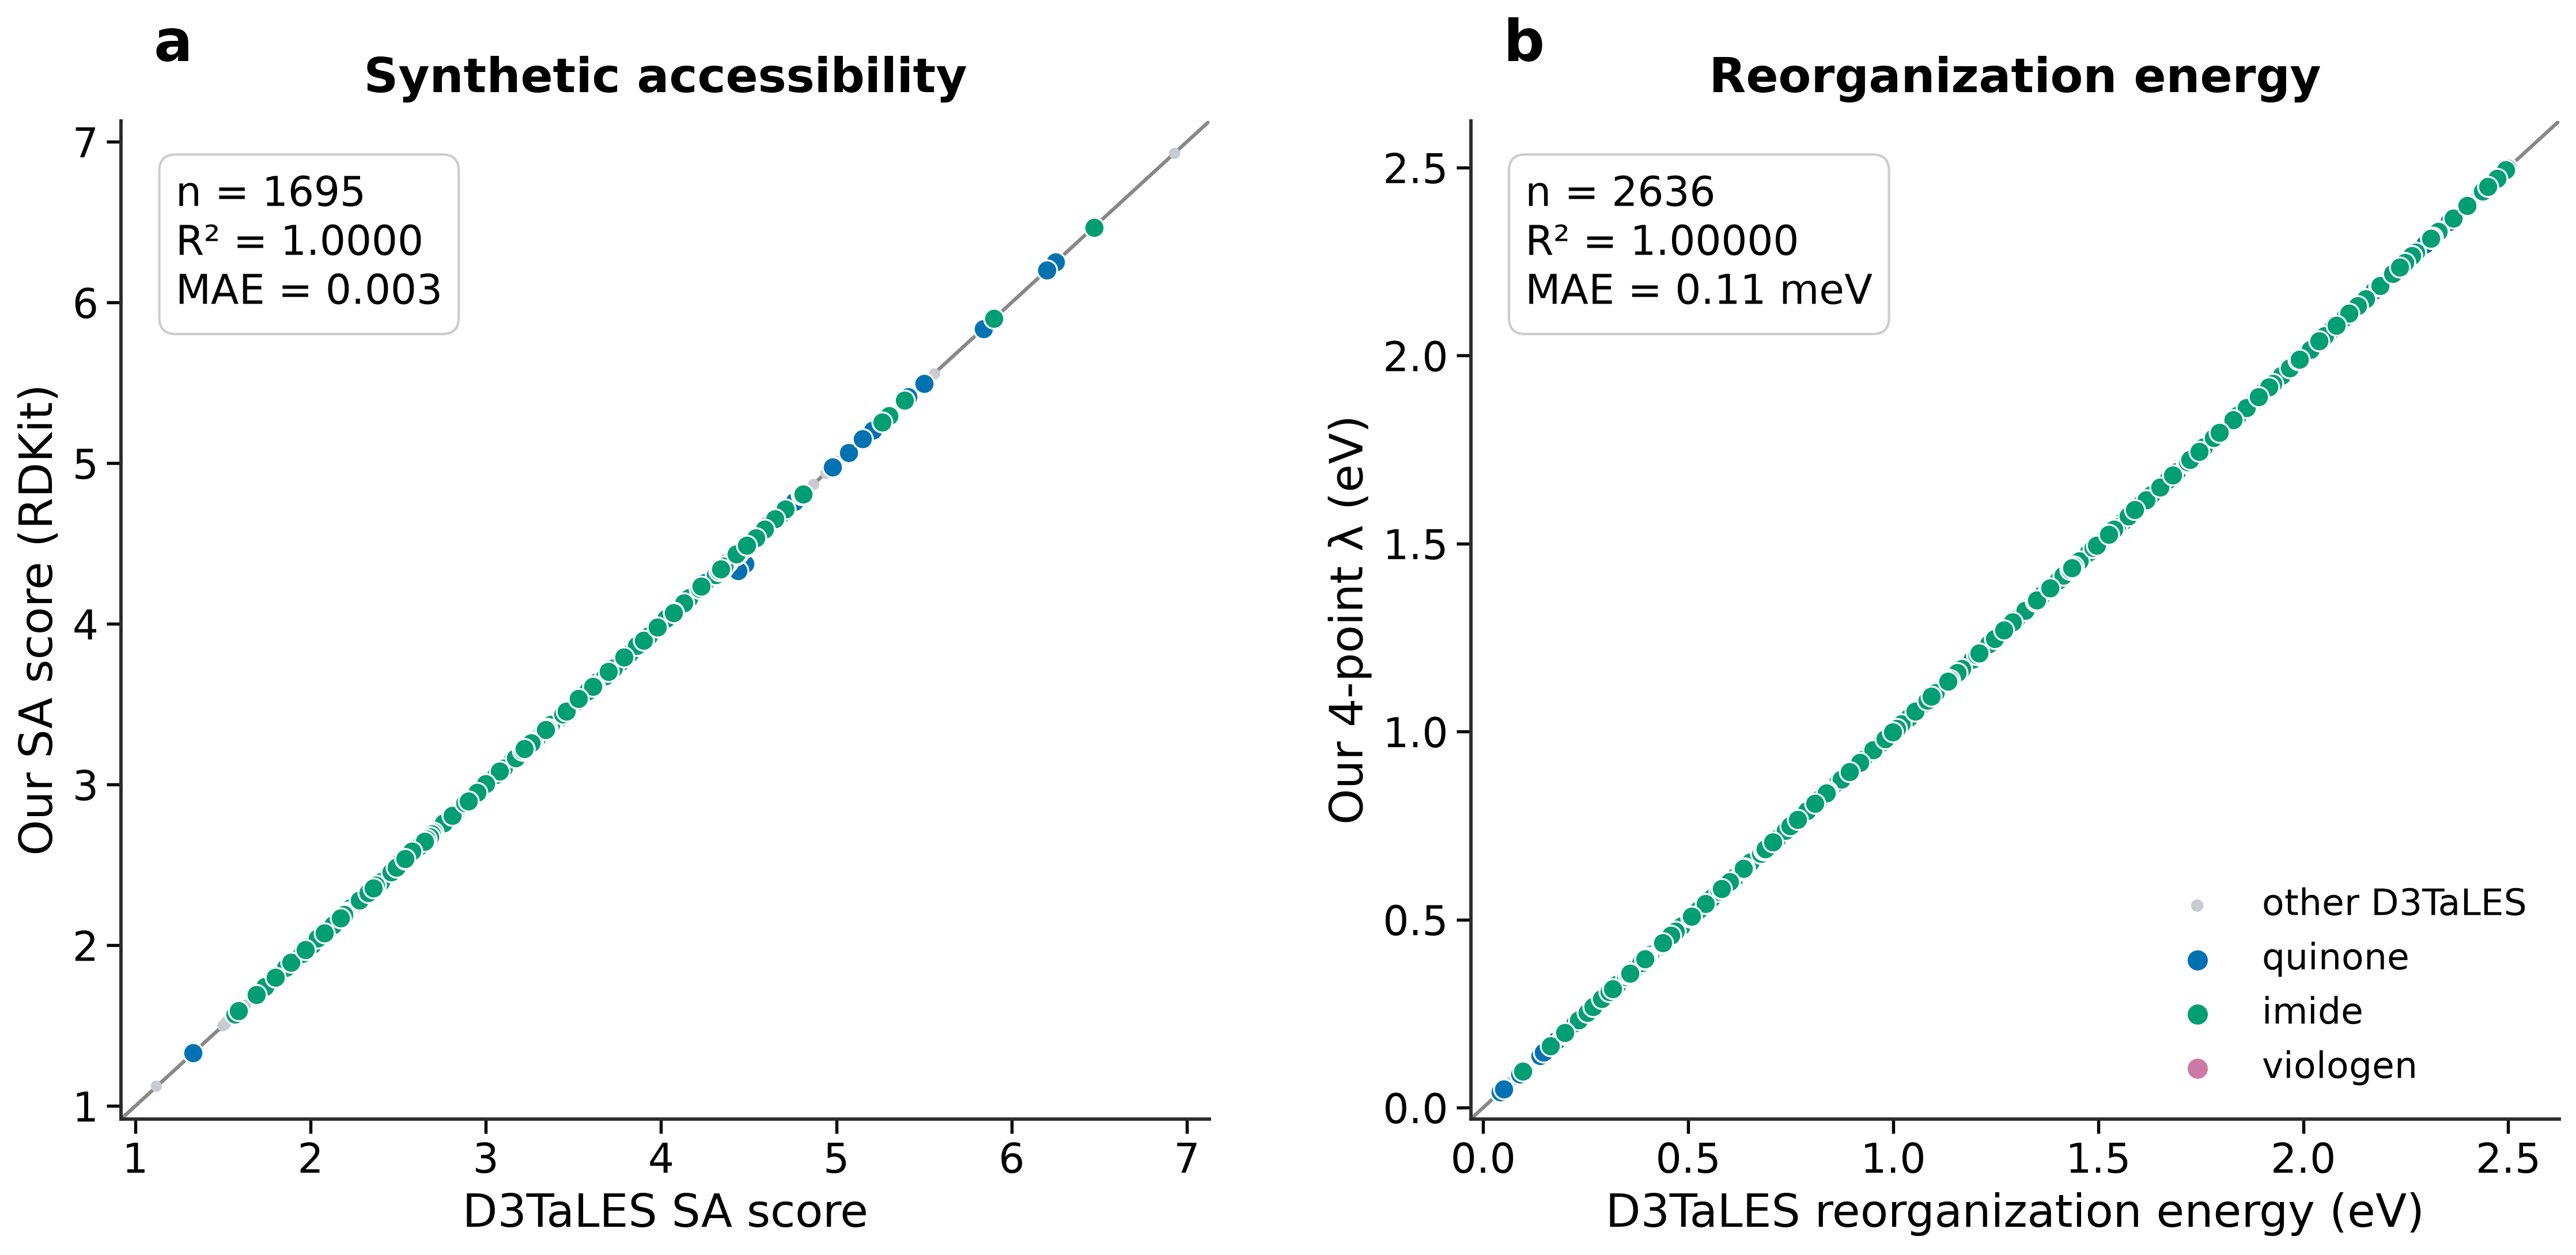
\includegraphics[width=\linewidth]{d3tales_validation.png}
      \end{center}
      \vspace{-1.5ex}
      \centering\footnotesize
      Independently reproduce D3TaLES's SA \& inner-sphere $\lambda$:
      \good{$R^2=1.0$} \ (SA $n{=}1695$; $\lambda$ $n{=}2636$; quinones \& imides highlighted).
    \end{column}
  \end{columns}
\end{frame}

% ---------------------------------------------------------------
\begin{frame}{Candidates: SA vs.\ reorganization energy}
  \begin{center}
  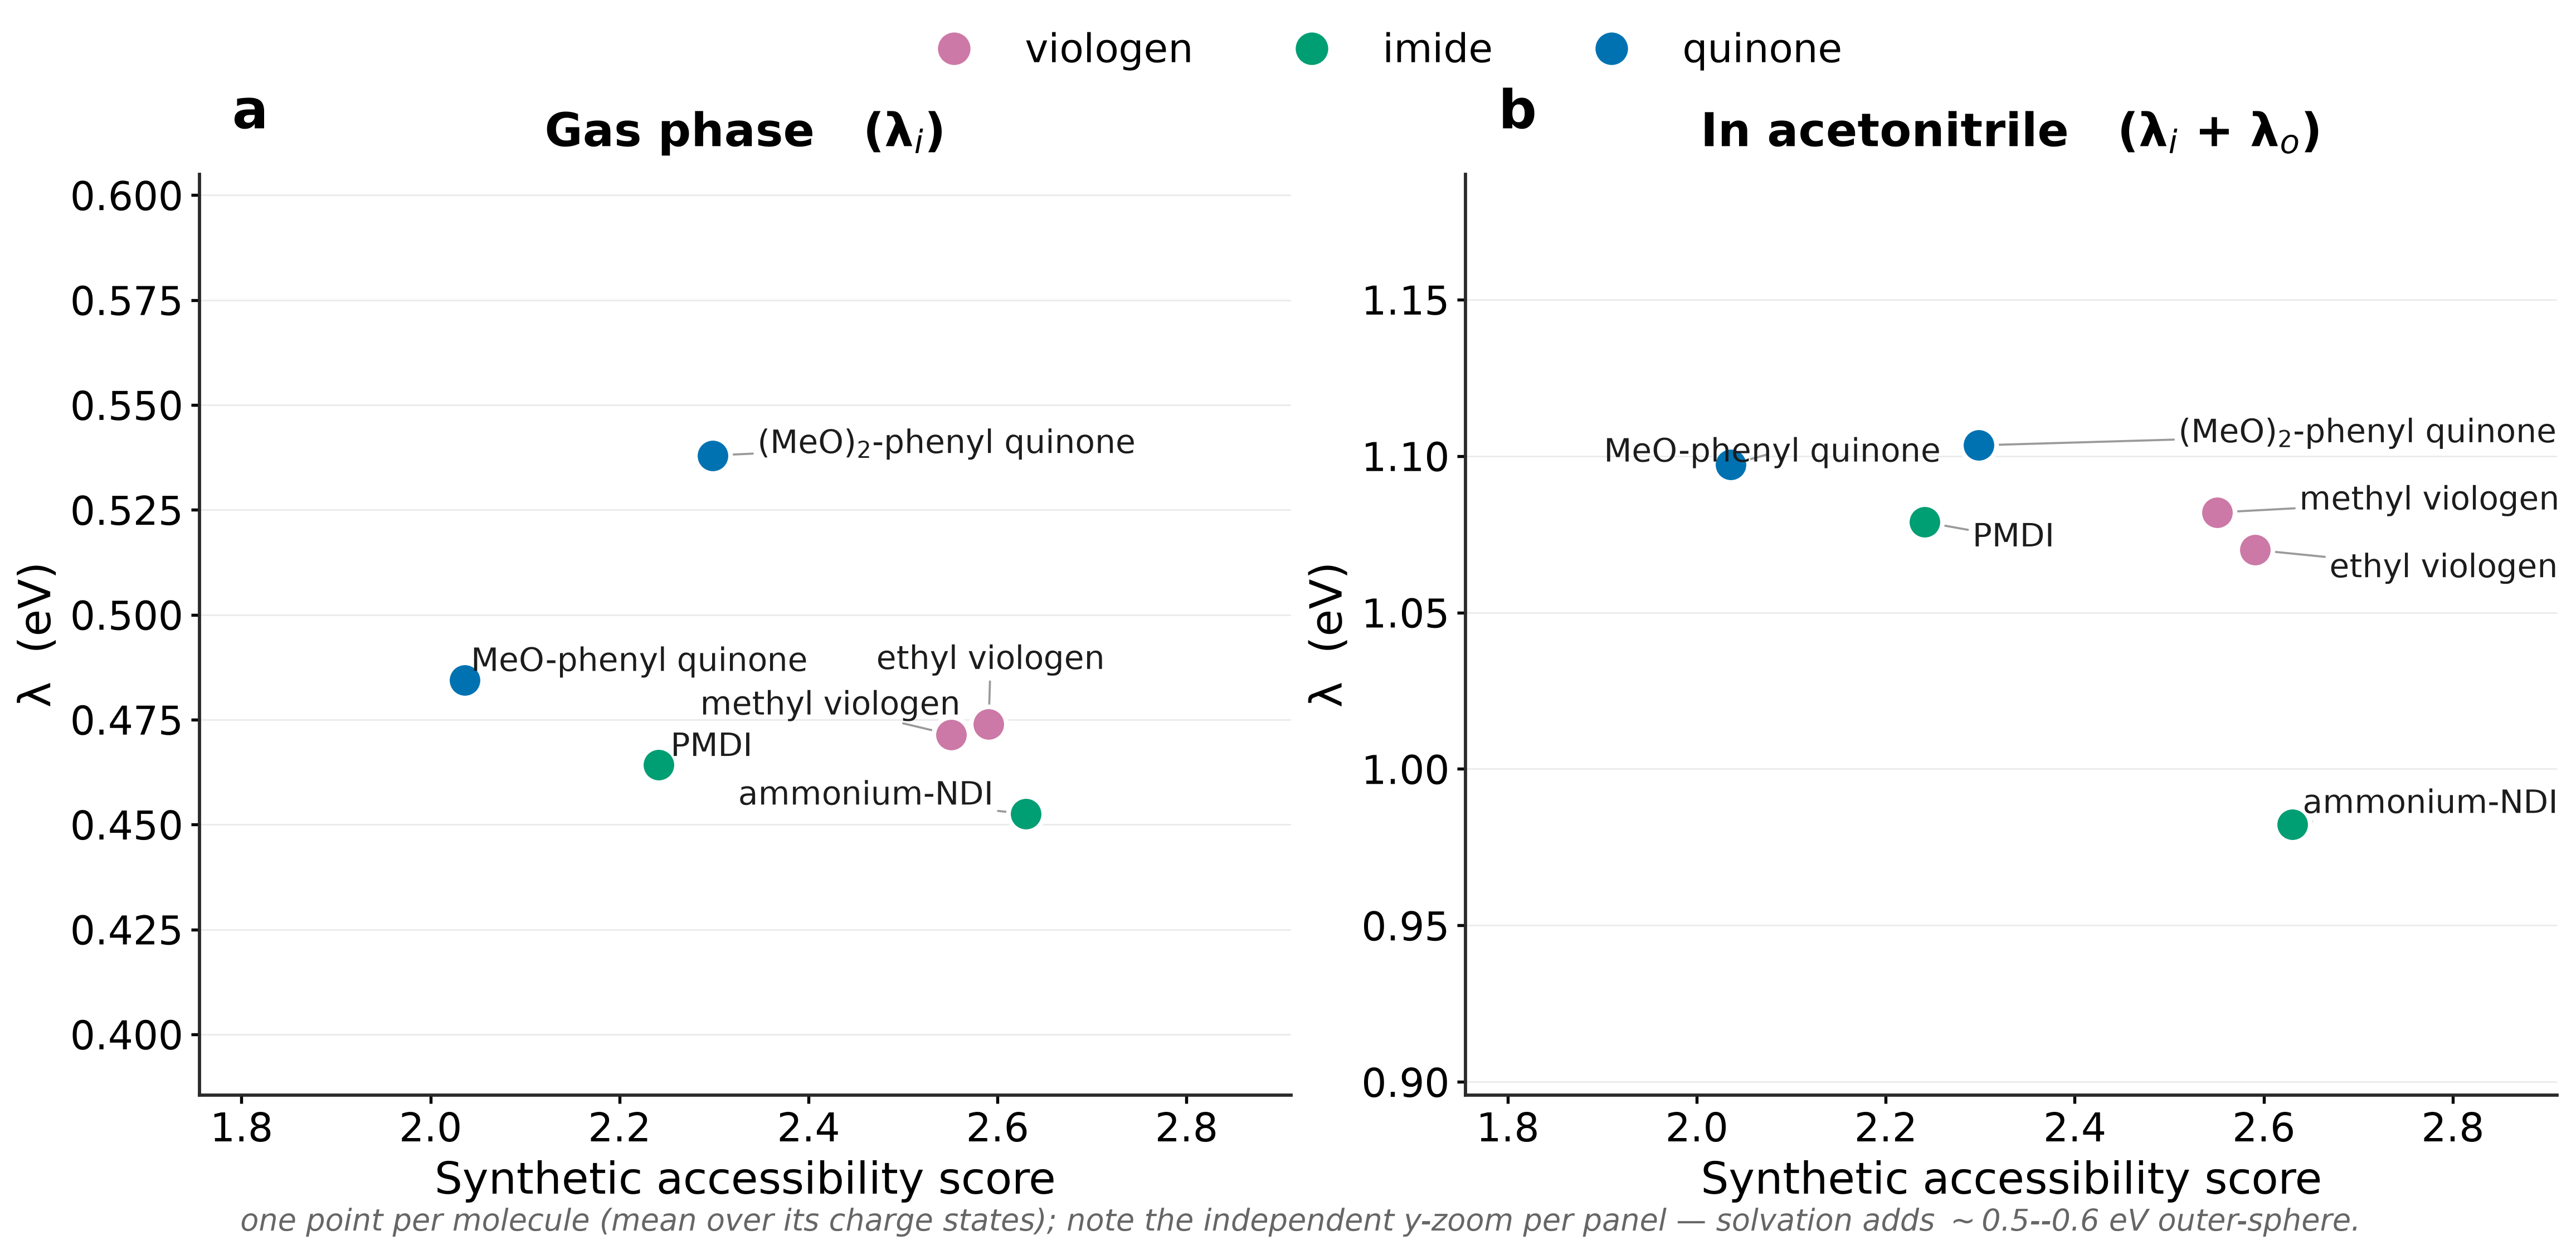
\includegraphics[width=0.99\textwidth]{candidates_sa_reorg.png}
  \end{center}
  \vspace{-1.5ex}
  \centering\scriptsize\textcolor{ink!70}{All six are \emph{grafted} model-compounds (redox core
  $+$ 4-methylbenzyl monomer proxy); short class names label them.}\par
  \vspace{0.4ex}
  \footnotesize
  \begin{columns}[T]
    \begin{column}{0.5\textwidth}
      \begin{itemize}\footnotesize
        \item one point per molecule (mean over its charge states); the six cluster tightly
              ($\lambda_i\!\approx$0.45--0.54 eV --- similar across families).
        \item \good{ammonium-NDI}: lowest $\lambda$ $\Rightarrow$ fastest ET; \hi{quinones} highest.
      \end{itemize}
    \end{column}
    \begin{column}{0.5\textwidth}
      \begin{itemize}\footnotesize
        \item gas $\to$ MeCN: $+\lambda_o$ lifts each point $\sim$0.5--0.6 eV (note per-panel y-zoom).
        \item $\lambda_i$ validated (D3TaLES $R^2{=}1.0$); $\lambda_o$ Marcus/Born estimate
              ($r_\text{hyd}$ caveat) --- read \emph{relative} trends.
      \end{itemize}
    \end{column}
  \end{columns}
\end{frame}

% ---------------------------------------------------------------
\begin{frame}{Functionalization $\times$ solvation: the 2$\times$2}
  \begin{columns}[T]
    \begin{column}{0.62\textwidth}
      \begin{center}
      
\includegraphics[width=\linewidth]{candidates_2x2_standalone_grafted.png}
      \end{center}
    \end{column}
    \begin{column}{0.38\textwidth}
      \footnotesize
      \textbf{Rows} = \hi{before} (standalone core) vs \hi{after} functionalization
      (grafted: redox core $+$ 4-methylbenzyl monomer handle).\\
      \textbf{Cols} = gas ($\lambda_i$) vs MeCN ($\lambda_i{+}\lambda_o$).
      \vspace{1.2ex}

      \textbf{Functionalization barely moves $\lambda_i$} --- $\pm$15--50 meV, mixed sign:
      \begin{itemize}\scriptsize
        \item viologens: $+$15 / $+$29 meV
        \item PMDI $+$22; \good{NDI $-$44}; quinones $0$ / \good{$-$52}
      \end{itemize}
      \vspace{0.5ex}
      \textbf{Solvation} adds a near-uniform \hi{$+$0.5--0.6 eV} ($\lambda_o$).
      \vspace{1.2ex}

      $\Rightarrow$ the \good{redox core sets $\lambda$}; the monomer handle is a small
      perturbation, so the cheap standalone $\lambda$ is a good predictor of the grafted value.
    \end{column}
  \end{columns}
  \vspace{0.3ex}
  \centering\scriptsize\textcolor{ink!70}{Standalone = ``before functionalization'' (methyl/
  methoxy cap); grafted = ``after'' (Merrifield benzylic handle). One point per molecule (mean
  over charge states).}
\end{frame}

% ---------------------------------------------------------------
\begin{frame}{What we learned (the durable lessons)}
  \begin{columns}[T]
    \begin{column}{0.5\textwidth}
      \textbf{\textcolor{good}{What works}}
      \begin{itemize}\footnotesize
        \item ranking (within charge class)
        \item xtb RRHO thermal (open-shell safe)
        \item disproportionation stability
        \item reorganization energy $\lambda$
        \item reversibility as filter + stability signal
        \item capacity ($n$, MW): exact
      \end{itemize}
    \end{column}
    \begin{column}{0.5\textwidth}
      \textbf{\textcolor{bad}{Negative results (saved effort)}}
      \begin{itemize}\footnotesize
        \item continuum ion-pairing: \bad{refuted} (spacing off by $\sim$11 V)
        \item explicit microsolvation (4 MeCN): \bad{no gain} for viologen
        \item absolute redox potential: capped $\sim$0.5 V
        \item dimerization absolute: \bad{unreliable} ($+2$ desolvation)
        \item solubility / crossover: proxies only
      \end{itemize}
    \end{column}
  \end{columns}
  \vspace{1ex}
  \begin{center}\small
  \textcolor{ink}{Corroborated by the metabolic-$\Delta G$ pipeline: 0.14 eV via isodesmic
  cancellation $\Rightarrow$ \hi{cancellation, not more physics, is the lever}.}
  \end{center}
\end{frame}

% ---------------------------------------------------------------
\begin{frame}{Putting it together: a tiered, multi-objective search}
  \begin{columns}[T]
    \begin{column}{0.46\textwidth}
      \textbf{Tiered funnel} (explicit solvation is a finisher, never for thousands):
      \begin{center}
      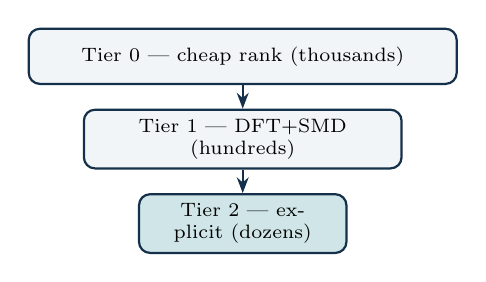
\begin{tikzpicture}[font=\scriptsize,node distance=3mm,
        t/.style={rectangle,rounded corners,draw=ink,fill=soft,thick,align=center,
                  minimum height=7mm}]
        \node[t,text width=52mm] (t0) {Tier 0 --- cheap rank (thousands)};
        \node[t,text width=38mm,below=of t0] (t1) {Tier 1 --- DFT+SMD (hundreds)};
        \node[t,text width=24mm,below=of t1,fill=teal!20] (t2) {Tier 2 --- explicit (dozens)};
        \draw[-{Stealth[length=2mm]},thick,ink] (t0)--(t1);
        \draw[-{Stealth[length=2mm]},thick,ink] (t1)--(t2);
      \end{tikzpicture}
      \end{center}
    \end{column}
    \begin{column}{0.54\textwidth}
      \textbf{Pareto scorecard --- built correctly}
      \begin{itemize}\footnotesize
        \item objectives = \good{trustworthy} axes only
              (capacity, $\lambda$, disprop.\ stability, ranked potential)
        \item proxies (solubility, SA, crossover) = \hi{filters}, not axes
        \item \textbf{reversibility} = hard pre-filter
        \item split \textbf{anolyte / catholyte} (potential isn't ``more is better'')
        \item \textbf{$\sigma$-aware} domination (don't rank within error)
        \item read the front against the \emph{raw} axes --- no scalarized score (arbitrary
              weights, $\sigma$-blind, pool-relative)
      \end{itemize}
    \end{column}
  \end{columns}
\end{frame}

% ---------------------------------------------------------------
\begin{frame}{Applying it: candidate scorecard $\rightarrow$ shortlist}
  \footnotesize
  $\sigma$-aware Pareto on the \hi{six grafted starting candidates} --- all fall in the
  \textbf{anolyte} pool (2e reductions / viologen reductions), all reversible, none gated out:
  \begin{columns}[T]
    \begin{column}{0.56\textwidth}
      \begin{table}\scriptsize
      \renewcommand{\arraystretch}{1.1}
      \begin{tabular}{lrrrrc}
        \toprule
        id & E$_\text{an}$ & Cap & $\lambda$ & $\Delta G_\text{d}$ & Par. \\
        \midrule
        pmdi                          & $-1.49$ & 160 & 0.46 & 73  & --- \\
        \good{mophquinone}$^\star$    & $-1.05$ & 176 & 0.48 & 101 & \good{Y} \\
        \good{viologen}$^\star$       & $-1.03$ & 194 & 0.47 & 52  & \good{Y} \\
        ethylviologen                 & $-1.03$ & 185 & 0.49 & 50  & --- \\
        dmophquinone                  & $-1.01$ & 147 & 0.54 & 101 & --- \\
        ndi\_ammonium                 & $-1.00$ & 114 & 0.45 & 29  & --- \\
        \bottomrule
      \end{tabular}
      \end{table}
      \scriptsize Ordered by primary axis (E$_\text{an}$). E$_\text{an}$ [V vs Fc], Cap
      [mAh/g], $\lambda$ [eV], $\Delta G_\text{d}$ (disprop.) [kJ/mol].
    \end{column}
    \begin{column}{0.44\textwidth}
      \scriptsize $^\star$ = Pareto-optimal ($\Rightarrow$ shortlist: \good{mophquinone},
      \good{viologen}). No scalarized ``figure of merit'': it needs arbitrary weights, ignores
      $\sigma$, and rescales with the candidate set. The front $+$ raw axes are the output.
      \vspace{1ex}

      \hi{$\sigma$-aware matters}: \textbf{pmdi} has the \emph{best voltage}
      ($-1.49$ V) yet is \emph{dropped} from the Pareto front --- its 0.44 V edge sits inside
      $\sigma_E\!\approx\!0.8$ V, so it is $\sigma$-dominated by the higher-capacity /
      more-stable mophquinone \& viologen.
      \vspace{1ex}

      $\Rightarrow$ across this tight set voltage is \emph{non-discriminating}; \good{capacity
      $+$ disproportionation stability $+$ $\lambda$} drive the ranking.
    \end{column}
  \end{columns}
  \vspace{0.5ex}
  \scriptsize\textcolor{ink!70}{Caveats surfaced automatically: the quinones' larger $\Delta
  G_\text{disp}$ (persistent semiquinone) offsets their lower capacity; viologen carries a
  flagged dimerization mode ($\Delta G_\text{dim}$ from earlier). All six are anolyte-side.}
\end{frame}

% ---------------------------------------------------------------
\begin{frame}{Current focus: six multi-electron starting candidates}
  \begin{center}
  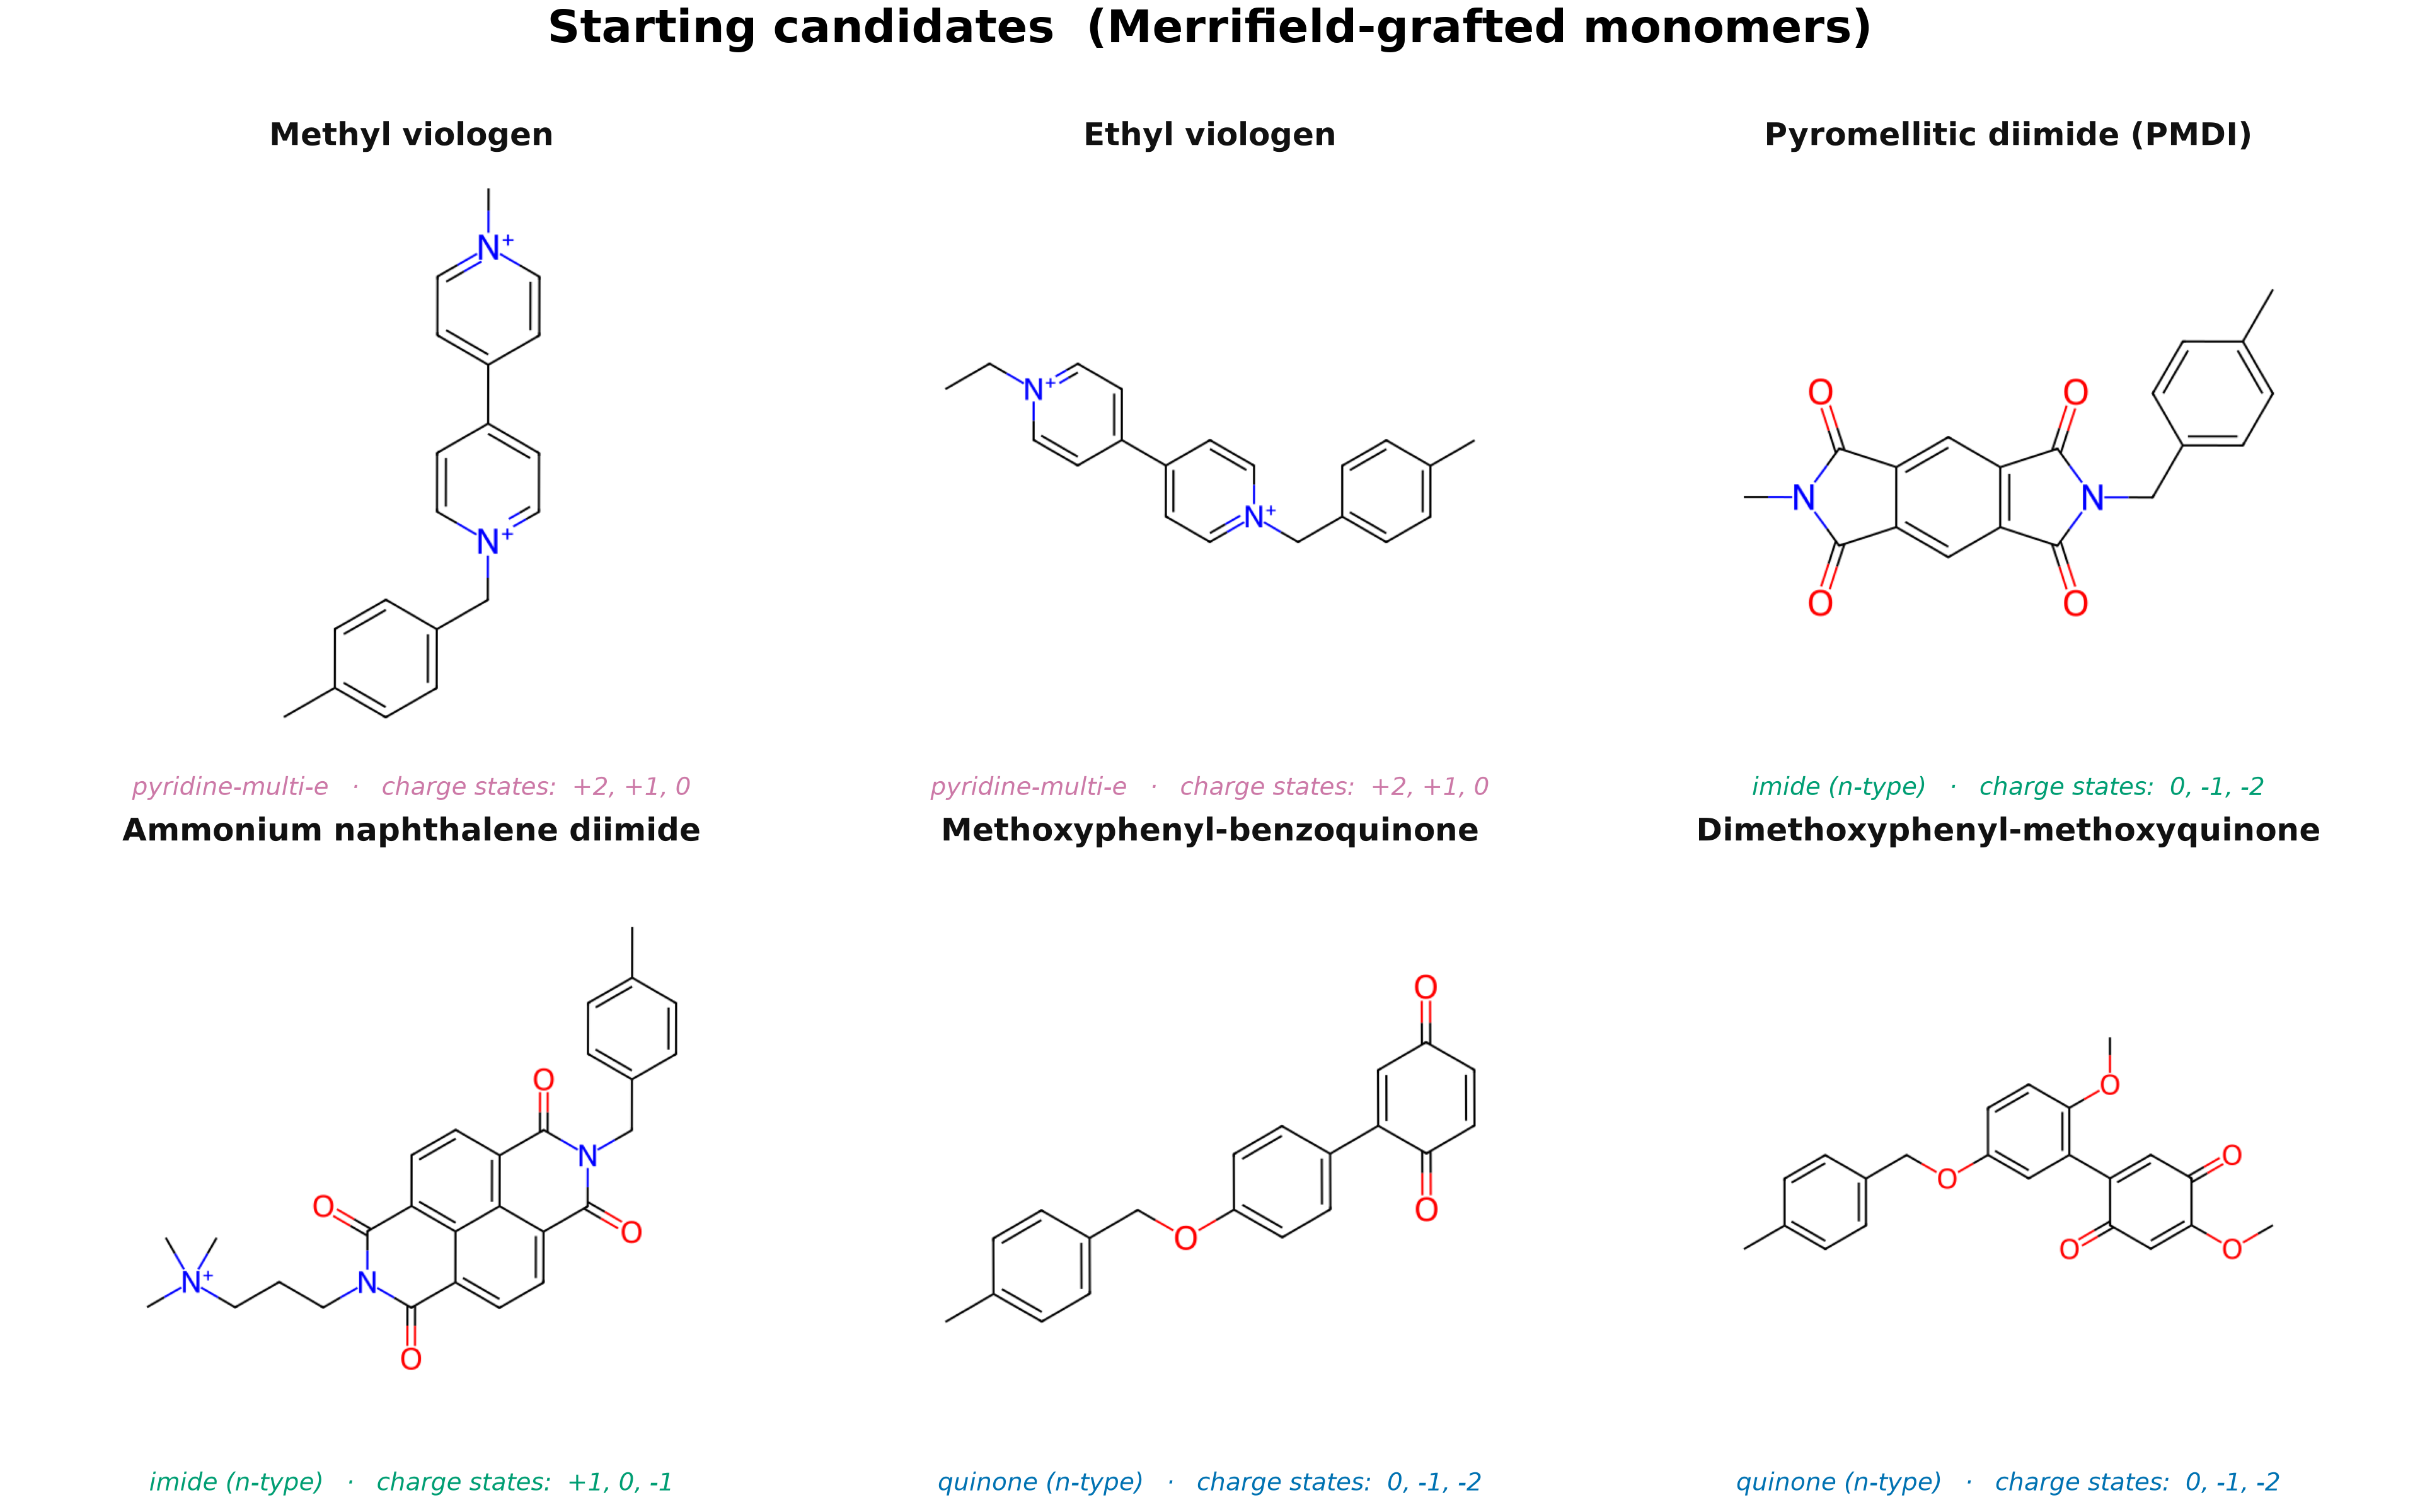
\includegraphics[width=0.92\textwidth]{molecules_starting_candidates.png}
  \end{center}
  \vspace{-0.5ex}
  \centering\footnotesize
  From \texttt{Candidates.xlsx}: two \hi{viologens}, two \hi{imides} (PMDI, NDI), two
  \hi{quinones} --- all \good{2-electron} (multi-charge) systems, grafted onto the Merrifield
  benzylic site. The \emph{imide} family is new; all six now entering the validated pipeline.
\end{frame}

% ---------------------------------------------------------------
\begin{frame}{Next steps}
  \textbf{\textcolor{good}{Done}}: all axes computed \& validated; unified $\sigma$-tagged
  scorecard; $\sigma$-aware Pareto engine; shortlist on the six grafted starting candidates
  (\good{mophquinone}, \good{viologen} Pareto-optimal).
  \vspace{1ex}
  \begin{enumerate}
    \item \hi{\textbf{Scale up discovery}} --- run the tiered funnel on a larger design space
          (functionalized variants + D3TaLES-mined pools), not just the current six.
    \item \textbf{Harden for scale} --- SCF-robustness patch ($\sim$20\% of jobs hit gradient
          non-convergence); needed before screening hundreds.
    \item \textbf{Broaden benchmarks} --- more two-wave molecules for stability; more OROP for
          the redox ranking, esp.\ per charge class.
    \item \textbf{Polymer effects} --- backbone/tether constraints \& inter-monomer
          dimerization (where the \emph{relative} dimerization ranking becomes key).
    \item \textbf{Absolute accuracy} (if needed) --- same-charge referencing to remove the
          per-class redox bias.
  \end{enumerate}
\end{frame}

% ---------------------------------------------------------------
\begin{frame}[plain]
  \vfill
  \begin{center}
    {\Large\textbf{\textcolor{ink}{Summary}}}\\[2ex]
    \begin{minipage}{0.85\textwidth}\centering
    We can \good{rank} redox candidates and screen \good{stability}, \good{kinetics}, and
    \good{reversibility} on a physics-based footing --- with each axis \hi{honestly labelled}
    by how far we can trust it.\\[2ex]
    The $\sigma$-aware scorecard \& Pareto engine are built and applied.
    Next: point the funnel at a larger design space.
    \end{minipage}
  \end{center}
  \vfill
\end{frame}

\end{document}
